\section{Resultados y discusión}
Con el objetivo de caracterizar el circuito incógnita, se realizaron mediciones de la tensión de entrada y salida a diferentes frecuencias, junto al desfasaje entre ambas señales, utilizando como señal de entrada una sinusoidal. Se estudió la respuesta del sistema en función de la frecuencia, en un rango de 10 \si{Hz} a 60 \si{\kilo\hertz}, realizando diagramas de Bode y de Nyquist para la impedancia del circuito, los cuales perimitieron determinar los distintos elementos que lo componen. Además, se propagaron pulsos de onda cuadrada a través del circuito, con el fin de estudiar su respuesta temporal y determinar las constantes de tiempo involucradas en el mismo. 

\subsection{Impedancia del sistema}
En primera instancia, se graficó el módulo de la impedancia $|Z|$ y la fase $\phi$ en función de la frecuencia $\omega$, obteniendo el diagrama de Bode que se presenta en la \autoref{Bode}. En el, es posible observar que el módulo de la impedancia disminuye al aumentar la frecuencia, a medida que el desfasaje entre las señales disminuye, lo que indica que el circuito se comporta como un filtro pasa bajos (o que el circuito es principalmente capacitivo?). Además, se observa una región de fase constante, entre los [160, 1700] \si{\hertz}, cuyo comportamiento se identificó como un elemento CPE. 

        \begin{figure}[H]
            \centering
            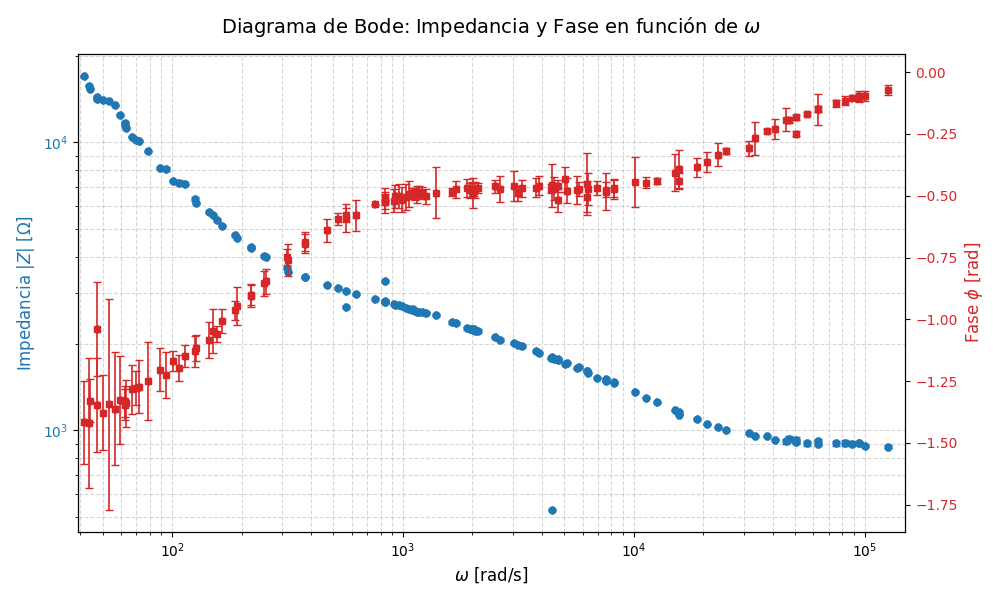
\includegraphics[width=0.5\textwidth]{Figuras/Bode.png}
            \caption{}
            \label{Bode}
        \end{figure}

Paralelamente, se graficó la impedancia en el plano complejo, obteniendo el diagrama de Nyquist que se presenta en la \autoref{Nyquist}. Se observa que el gráfico inicia en el eje real, donde la impedancia es puramente resistiva, con un valor de apróximadamente \SI{1}{\kilo\ohm}. Luego, a medida que disminuye la frecuencia, el valor del eje imaginario aumenta, de manera que el digrama se curva formando una fracción de circunferencia, lo que indica un comportamiento similar al de un circuito RC en paralelo. No obstante, el diagrama no forma un semicirculo perfecto, sino que es interrumpido por una recta (semirrecta) de pendiente distinta a 0 o 1, la cual resulta característica de un elemento de fase constante. Finalmente, a frecuencias suficientemente bajas, los datos experimentales crecen abruptamente sobre el eje imaginario, lo que indica un comportamiento capacitivo predominante.

\begin{figure}[H]
    \centering
     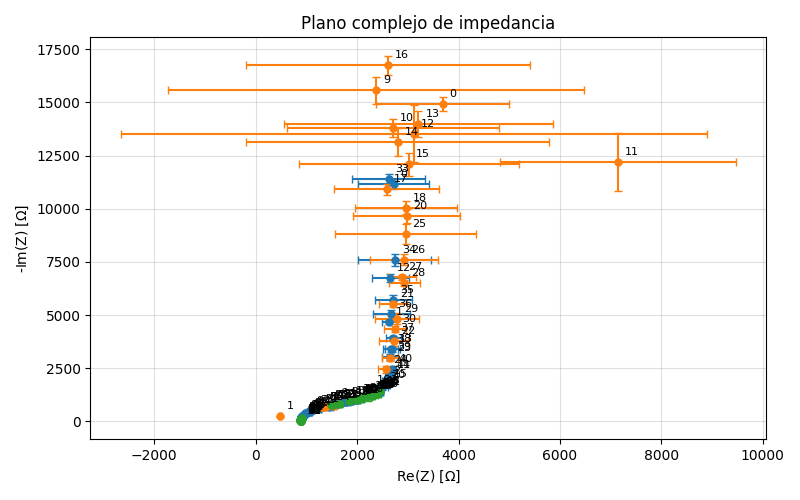
\includegraphics[width=0.5\textwidth]{Figuras/Nyquist.png}
            \caption{}
            \label{Nyquist}
\end{figure}

En base a las observaciones realizadas sobre los diagramas de Bode y Nyquist, se propuso un modelo equivalente para el circuito (referenciar al diagrama de métodos), el cual fue ajustado a los datos experimentales representados en el diagrama de Nyquist (Ver figura \ref{Nyquist-modelo}). 

\begin{figure}
    \centering
     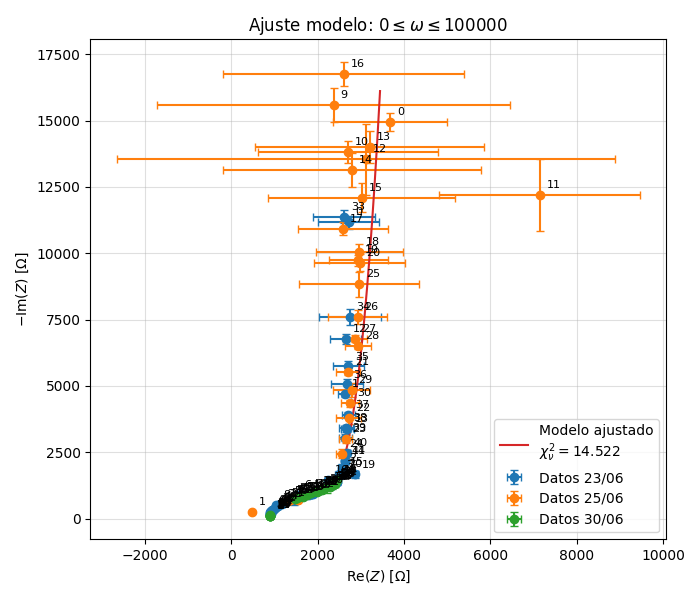
\includegraphics[width=0.5\textwidth]{Figuras/Nyquist-modelo.png}
            \caption{}
            \label{Nyquist-modelo}
\end{figure}

A partir del ajuste, fue posible determinar los valores de los distintos elementos que componen el circuito, los cuales se presentan en la autoref{tabla-elementos}.

\subsection{Determinación de \texorpdfstring{$\tau$}{tau} utilizando pulsos cuadrados}
Se registró la respuesta del circuito frente a la propagación de pulsos de onda cuadrada, con el objetivo de determinar las constantes de tiempo involucradas en el mismo. Se realizaron mediciones de la tensión de salida en función del tiempo, para diferentes frecuencias de la señal de entrada. Por cada frecuencia, se registraron tres series que contengan al menos 6 pulsos, los cuales se ajustaron según la ecuación (acá o en métodos), 
\begin{equation}
    V(t) = C_i + A_i e^{-t/\tau}
    \label{ajuste-pulsoscuadrados}
\end{equation}
donde i indica el número de pulso que se muestra en la pantalla (Ver \autoref{pulsos}). 

\begin{figure}[H]
    \centering
     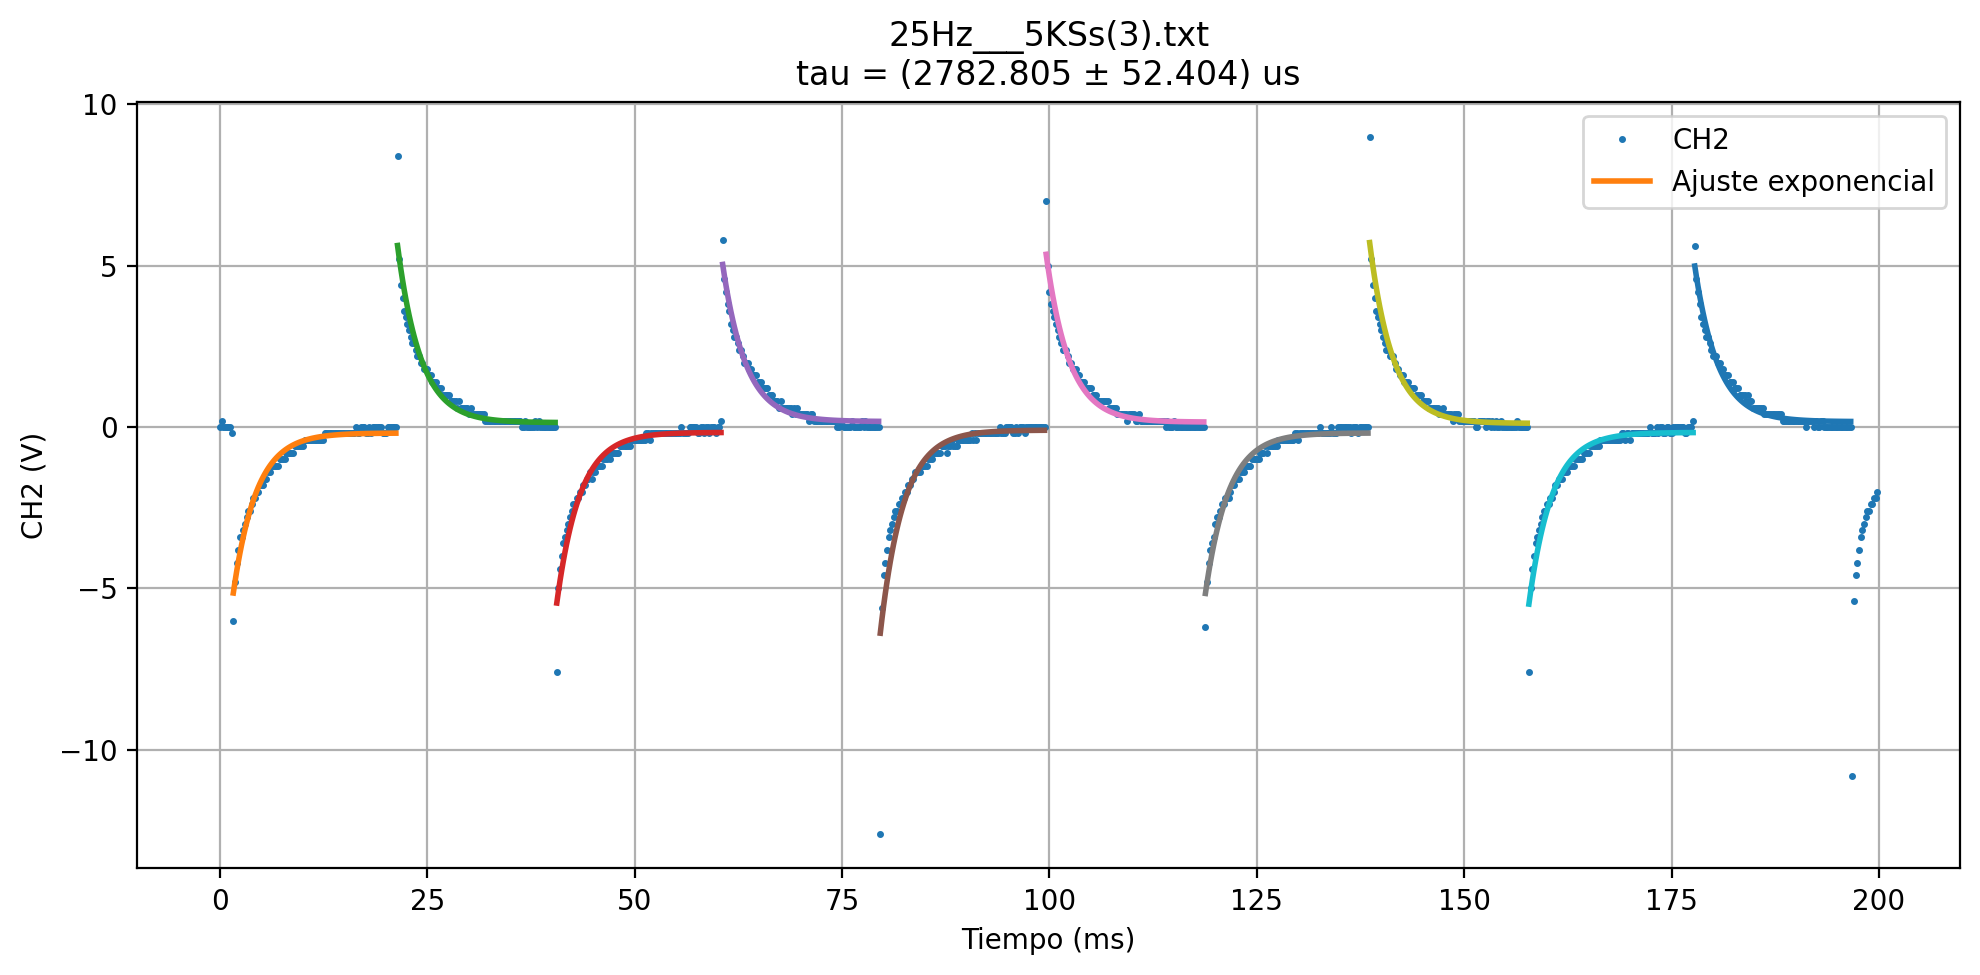
\includegraphics[width=0.5\textwidth]{Figuras/pulsos.png}
            \caption{}
            \label{pulsos}
            \end{figure}